%% ============================================================
%% CurricuMap — SoftwareX Original Software Publication (revision 1)
%% Elsevier elsarticle, following the SoftwareX OSP template (2026).
%% Compile: pdflatex -> bibtex -> pdflatex -> pdflatex
%% ============================================================
\documentclass[preprint,12pt,a4paper]{elsarticle}
\usepackage[T1]{fontenc}
\usepackage{lmodern}
\usepackage{graphicx}
\usepackage{xurl}
\usepackage{booktabs}
\usepackage{array}
\usepackage{tabularx}
\usepackage{float}
\newcolumntype{L}[1]{>{\raggedright\arraybackslash}p{#1}}
\newcolumntype{Y}{>{\raggedright\arraybackslash}X}
\usepackage{xcolor}
\usepackage{upquote}
\usepackage{listings}
\usepackage{tikz}
\usetikzlibrary{arrows.meta,positioning,calc}
\usepackage[hidelinks]{hyperref}
\emergencystretch=2em
\newcommand{\tbd}[1]{\textbf{\textcolor{red}{#1}}}
% Generated by validation/paper_numbers.py -- do not edit by hand.
\newcommand{\nTitles}{143}
\newcommand{\nExact}{128}
\newcommand{\nVariant}{10}
\newcommand{\nUnseen}{5}
\newcommand{\nClusters}{114}
\newcommand{\clusterLo}{96.7}
\newcommand{\nVariantLoose}{4}
\newcommand{\nUnseenW}{five}
\newcommand{\nVariantLooseW}{four}
\newcommand{\vOneCov}{49.0}
\newcommand{\vOneAcc}{40.6}
\newcommand{\vOneAccMin}{40.6}
\newcommand{\vOneAccMax}{40.6}
\newcommand{\vOneKappa}{0.313}
\newcommand{\vOneOff}{45.5}
\newcommand{\vOneCorrect}{58}
\newcommand{\vOneAssigned}{70}
\newcommand{\vOneFlagged}{73}
\newcommand{\vOneWrong}{12}
\newcommand{\vOneExact}{50}
\newcommand{\vOneVariant}{4}
\newcommand{\vOneUnseen}{4}
\newcommand{\vOneP}{$<$0.001}
\newcommand{\vOnePt}{$p<0.001$}
\newcommand{\vOnePMaxUp}{0.001}
\newcommand{\vOneIdentical}{100.0}
\newcommand{\vOneRuns}{1}
\newcommand{\vOneRunsW}{one}
\newcommand{\vOneWrongW}{12}
\newcommand{\vTwoCov}{100.0}
\newcommand{\vTwoAcc}{100.0}
\newcommand{\vTwoAccMin}{100.0}
\newcommand{\vTwoAccMax}{100.0}
\newcommand{\vTwoKappa}{1.000}
\newcommand{\vTwoOff}{99.3}
\newcommand{\vTwoCorrect}{143}
\newcommand{\vTwoAssigned}{143}
\newcommand{\vTwoFlagged}{0}
\newcommand{\vTwoWrong}{0}
\newcommand{\vTwoExact}{128}
\newcommand{\vTwoVariant}{10}
\newcommand{\vTwoUnseen}{5}
\newcommand{\vTwoP}{1.000}
\newcommand{\vTwoPt}{$p=1.000$}
\newcommand{\vTwoPMaxUp}{1.000}
\newcommand{\vTwoIdentical}{100.0}
\newcommand{\vTwoRuns}{1}
\newcommand{\vTwoRunsW}{one}
\newcommand{\vTwoWrongW}{zero}
\newcommand{\lookCov}{89.5}
\newcommand{\lookAcc}{89.5}
\newcommand{\lookAccMin}{89.5}
\newcommand{\lookAccMax}{89.5}
\newcommand{\lookKappa}{0.858}
\newcommand{\lookOff}{88.8}
\newcommand{\lookCorrect}{128}
\newcommand{\lookAssigned}{128}
\newcommand{\lookFlagged}{15}
\newcommand{\lookWrong}{0}
\newcommand{\lookExact}{128}
\newcommand{\lookVariant}{0}
\newcommand{\lookUnseen}{0}
\newcommand{\lookP}{$<$0.001}
\newcommand{\lookPt}{$p<0.001$}
\newcommand{\lookPMaxUp}{0.001}
\newcommand{\lookIdentical}{100.0}
\newcommand{\lookRuns}{1}
\newcommand{\lookRunsW}{one}
\newcommand{\lookWrongW}{zero}
\newcommand{\strNNCov}{100.0}
\newcommand{\strNNAcc}{98.6}
\newcommand{\strNNAccMin}{98.6}
\newcommand{\strNNAccMax}{98.6}
\newcommand{\strNNKappa}{0.980}
\newcommand{\strNNOff}{97.9}
\newcommand{\strNNCorrect}{141}
\newcommand{\strNNAssigned}{143}
\newcommand{\strNNFlagged}{0}
\newcommand{\strNNWrong}{2}
\newcommand{\strNNExact}{128}
\newcommand{\strNNVariant}{10}
\newcommand{\strNNUnseen}{3}
\newcommand{\strNNP}{0.500}
\newcommand{\strNNPt}{$p=0.500$}
\newcommand{\strNNPMaxUp}{0.500}
\newcommand{\strNNIdentical}{100.0}
\newcommand{\strNNRuns}{1}
\newcommand{\strNNRunsW}{one}
\newcommand{\strNNWrongW}{two}
\newcommand{\chrCov}{100.0}
\newcommand{\chrAcc}{100.0}
\newcommand{\chrAccMin}{100.0}
\newcommand{\chrAccMax}{100.0}
\newcommand{\chrKappa}{1.000}
\newcommand{\chrOff}{99.3}
\newcommand{\chrCorrect}{143}
\newcommand{\chrAssigned}{143}
\newcommand{\chrFlagged}{0}
\newcommand{\chrWrong}{0}
\newcommand{\chrExact}{128}
\newcommand{\chrVariant}{10}
\newcommand{\chrUnseen}{5}
\newcommand{\chrP}{1.000}
\newcommand{\chrPt}{$p=1.000$}
\newcommand{\chrPMaxUp}{1.000}
\newcommand{\chrIdentical}{100.0}
\newcommand{\chrRuns}{1}
\newcommand{\chrRunsW}{one}
\newcommand{\chrWrongW}{zero}
\newcommand{\eZSCov}{100.0}
\newcommand{\eZSAcc}{68.5}
\newcommand{\eZSAccMin}{68.5}
\newcommand{\eZSAccMax}{68.5}
\newcommand{\eZSKappa}{0.569}
\newcommand{\eZSOff}{86.0}
\newcommand{\eZSCorrect}{98}
\newcommand{\eZSAssigned}{143}
\newcommand{\eZSFlagged}{0}
\newcommand{\eZSWrong}{45}
\newcommand{\eZSExact}{92}
\newcommand{\eZSVariant}{3}
\newcommand{\eZSUnseen}{3}
\newcommand{\eZSP}{$<$0.001}
\newcommand{\eZSPt}{$p<0.001$}
\newcommand{\eZSPMaxUp}{0.001}
\newcommand{\eZSIdentical}{100.0}
\newcommand{\eZSRuns}{1}
\newcommand{\eZSRunsW}{one}
\newcommand{\eZSWrongW}{45}
\newcommand{\eNNCov}{100.0}
\newcommand{\eNNAcc}{100.0}
\newcommand{\eNNAccMin}{100.0}
\newcommand{\eNNAccMax}{100.0}
\newcommand{\eNNKappa}{1.000}
\newcommand{\eNNOff}{99.3}
\newcommand{\eNNCorrect}{143}
\newcommand{\eNNAssigned}{143}
\newcommand{\eNNFlagged}{0}
\newcommand{\eNNWrong}{0}
\newcommand{\eNNExact}{128}
\newcommand{\eNNVariant}{10}
\newcommand{\eNNUnseen}{5}
\newcommand{\eNNP}{1.000}
\newcommand{\eNNPt}{$p=1.000$}
\newcommand{\eNNPMaxUp}{1.000}
\newcommand{\eNNIdentical}{100.0}
\newcommand{\eNNRuns}{1}
\newcommand{\eNNRunsW}{one}
\newcommand{\eNNWrongW}{zero}
\newcommand{\gmZSgCov}{100.0}
\newcommand{\gmZSgAcc}{91.6}
\newcommand{\gmZSgAccMin}{91.6}
\newcommand{\gmZSgAccMax}{91.6}
\newcommand{\gmZSgKappa}{0.882}
\newcommand{\gmZSgOff}{94.4}
\newcommand{\gmZSgCorrect}{131}
\newcommand{\gmZSgAssigned}{143}
\newcommand{\gmZSgFlagged}{0}
\newcommand{\gmZSgWrong}{12}
\newcommand{\gmZSgExact}{118}
\newcommand{\gmZSgVariant}{8}
\newcommand{\gmZSgUnseen}{5}
\newcommand{\gmZSgP}{$<$0.001}
\newcommand{\gmZSgPt}{$p<0.001$}
\newcommand{\gmZSgPMaxUp}{0.001}
\newcommand{\gmZSgIdentical}{100.0}
\newcommand{\gmZSgRuns}{1}
\newcommand{\gmZSgRunsW}{one}
\newcommand{\gmZSgWrongW}{12}
\newcommand{\gmZSCov}{100.0}
\newcommand{\gmZSAcc}{91.7}
\newcommand{\gmZSAccMin}{88.1}
\newcommand{\gmZSAccMax}{94.4}
\newcommand{\gmZSKappa}{0.883}
\newcommand{\gmZSOff}{95.1}
\newcommand{\gmZSCorrect}{131}
\newcommand{\gmZSAssigned}{143}
\newcommand{\gmZSFlagged}{0}
\newcommand{\gmZSWrong}{12}
\newcommand{\gmZSExact}{120}
\newcommand{\gmZSVariant}{8}
\newcommand{\gmZSUnseen}{5}
\newcommand{\gmZSP}{0.002}
\newcommand{\gmZSPt}{$p=0.002$}
\newcommand{\gmZSPMaxUp}{0.008}
\newcommand{\gmZSIdentical}{90.9}
\newcommand{\gmZSRuns}{5}
\newcommand{\gmZSRunsW}{five}
\newcommand{\gmZSWrongW}{12}
\newcommand{\gmFSgCov}{100.0}
\newcommand{\gmFSgAcc}{100.0}
\newcommand{\gmFSgAccMin}{100.0}
\newcommand{\gmFSgAccMax}{100.0}
\newcommand{\gmFSgKappa}{1.000}
\newcommand{\gmFSgOff}{99.3}
\newcommand{\gmFSgCorrect}{143}
\newcommand{\gmFSgAssigned}{143}
\newcommand{\gmFSgFlagged}{0}
\newcommand{\gmFSgWrong}{0}
\newcommand{\gmFSgExact}{128}
\newcommand{\gmFSgVariant}{10}
\newcommand{\gmFSgUnseen}{5}
\newcommand{\gmFSgP}{1.000}
\newcommand{\gmFSgPt}{$p=1.000$}
\newcommand{\gmFSgPMaxUp}{1.000}
\newcommand{\gmFSgIdentical}{100.0}
\newcommand{\gmFSgRuns}{1}
\newcommand{\gmFSgRunsW}{one}
\newcommand{\gmFSgWrongW}{zero}
\newcommand{\gmFSCov}{100.0}
\newcommand{\gmFSAcc}{99.9}
\newcommand{\gmFSAccMin}{99.3}
\newcommand{\gmFSAccMax}{100.0}
\newcommand{\gmFSKappa}{0.998}
\newcommand{\gmFSOff}{99.2}
\newcommand{\gmFSCorrect}{143}
\newcommand{\gmFSAssigned}{143}
\newcommand{\gmFSFlagged}{0}
\newcommand{\gmFSWrong}{0}
\newcommand{\gmFSExact}{128}
\newcommand{\gmFSVariant}{10}
\newcommand{\gmFSUnseen}{5}
\newcommand{\gmFSP}{1.000}
\newcommand{\gmFSPt}{$p=1.000$}
\newcommand{\gmFSPMaxUp}{1.000}
\newcommand{\gmFSIdentical}{99.3}
\newcommand{\gmFSRuns}{5}
\newcommand{\gmFSRunsW}{five}
\newcommand{\gmFSWrongW}{zero}
\newcommand{\clZSCov}{100.0}
\newcommand{\clZSAcc}{98.6}
\newcommand{\clZSAccMin}{98.6}
\newcommand{\clZSAccMax}{98.6}
\newcommand{\clZSKappa}{0.980}
\newcommand{\clZSOff}{97.9}
\newcommand{\clZSCorrect}{141}
\newcommand{\clZSAssigned}{143}
\newcommand{\clZSFlagged}{0}
\newcommand{\clZSWrong}{2}
\newcommand{\clZSExact}{126}
\newcommand{\clZSVariant}{10}
\newcommand{\clZSUnseen}{5}
\newcommand{\clZSP}{0.500}
\newcommand{\clZSPt}{$p=0.500$}
\newcommand{\clZSPMaxUp}{0.500}
\newcommand{\clZSIdentical}{100.0}
\newcommand{\clZSRuns}{5}
\newcommand{\clZSRunsW}{five}
\newcommand{\clZSWrongW}{two}
\newcommand{\clFSCov}{100.0}
\newcommand{\clFSAcc}{100.0}
\newcommand{\clFSAccMin}{100.0}
\newcommand{\clFSAccMax}{100.0}
\newcommand{\clFSKappa}{1.000}
\newcommand{\clFSOff}{99.3}
\newcommand{\clFSCorrect}{143}
\newcommand{\clFSAssigned}{143}
\newcommand{\clFSFlagged}{0}
\newcommand{\clFSWrong}{0}
\newcommand{\clFSExact}{128}
\newcommand{\clFSVariant}{10}
\newcommand{\clFSUnseen}{5}
\newcommand{\clFSP}{1.000}
\newcommand{\clFSPt}{$p=1.000$}
\newcommand{\clFSPMaxUp}{1.000}
\newcommand{\clFSIdentical}{100.0}
\newcommand{\clFSRuns}{5}
\newcommand{\clFSRunsW}{five}
\newcommand{\clFSWrongW}{zero}
\newcommand{\listAccMin}{98.6}
\newcommand{\listAccMax}{100.0}
\newcommand{\listPMin}{0.500}
\newcommand{\nAmbiguous}{10}
\newcommand{\eltKwOnlyCorrect}{113}
\newcommand{\eltKwOnlyEntries}{158}
\newcommand{\eltRules}{9}
\newcommand{\eltKeywords}{53}
\newcommand{\eltRegexes}{63}
\newcommand{\eltOverrides}{0}
\newcommand{\eltYamllines}{159}
\newcommand{\eltOldRules}{5}
\newcommand{\eltOldKeywords}{34}
\newcommand{\eltOldRegexes}{0}
\newcommand{\eltOldOverrides}{0}
\newcommand{\eltOldYamllines}{25}

% Generated by benchmarks/benchmark.py -- do not edit by hand.
\newcommand{\benchMaxRecords}{1.5}
\newcommand{\benchMaxStudents}{100{,}000}
\newcommand{\benchMaxTime}{3.19}
\newcommand{\benchMaxMem}{412}
\newcommand{\benchStartup}{0.5}

% Generated by paper/software_numbers.py -- do not edit by hand.
\newcommand{\nTests}{206}
\newcommand{\covPct}{99}
\newcommand{\exRecords}{878}
\newcommand{\exCourses}{15}
\newcommand{\exMissMin}{6.7}
\newcommand{\exMissMax}{15.0}
\newcommand{\exAlphaLS}{.769}
\newcommand{\exAlphaPed}{.767}
\newcommand{\exAlphaLing}{.761}
\newcommand{\exAlphaLit}{.819}
\newcommand{\exAlphaGE}{.781}

\lstset{basicstyle=\ttfamily\footnotesize,columns=fullflexible,keepspaces=true,breaklines=true,upquote=true,
  frame=single,framesep=3pt,xleftmargin=4pt,xrightmargin=4pt,aboveskip=6pt,belowskip=6pt,
  literate={İ}{{\.I}}1 {ı}{{\i}}1 {ş}{{\c{s}}}1 {Ş}{{\c{S}}}1 {ğ}{{\u{g}}}1 {Ğ}{{\u{G}}}1
           {ç}{{\c{c}}}1 {Ç}{{\c{C}}}1 {ö}{{\"o}}1 {Ö}{{\"O}}1 {ü}{{\"u}}1 {Ü}{{\"U}}1 {â}{{\^a}}1}
\renewcommand{\lstlistingname}{Listing}

\journal{SoftwareX}

\begin{document}
\begin{frontmatter}

\title{CurricuMap: an open-source Python pipeline for converting registrar transcript exports into auditable student-by-competency-domain matrices}

\author[iue]{Tar{\i}k K\"u\c{c}\"ukdeniz\corref{cor1}}
\ead{tkdeniz@iuc.edu.tr}
\author[elt]{Tuncer Can}
\cortext[cor1]{Corresponding author}

\affiliation[iue]{organization={Department of Industrial Engineering, Faculty of Engineering, \.Istanbul University-Cerrahpa\c{s}a},
            city={\.Istanbul}, country={T\"urkiye}}
\affiliation[elt]{organization={Department of English Language Teaching, Hasan Ali Y\"ucel Faculty of Education, \.Istanbul University-Cerrahpa\c{s}a},
            city={\.Istanbul}, country={T\"urkiye}}

\begin{abstract}
Competency-level learning analytics needs a student-by-competency-domain matrix, but institutions hold registrar transcript exports, and the conversion is usually an undocumented spreadsheet step. CurricuMap is an open-source Python library and command-line tool that performs it. The course-to-domain mapping is a declarative, schema-validated YAML specification of ordered keyword and regular-expression rules and explicit overrides; every assignment records its provenance, unmatched courses are flagged, and an audit reports coverage and reliability. On the \nTitles{} course titles of a Turkish teacher-education programme, a taxonomy written by language-model agents from the labelled course list of the national curriculum, unedited and frozen before testing, assigned every title as its labelling convention prescribes, as did the best baselines given the same list.
\end{abstract}

\begin{keyword}
Learning analytics \sep Curriculum mapping \sep Competency assessment \sep Data provenance
\end{keyword}

\end{frontmatter}

%% ============================================================
\section*{Required Metadata}
\label{metadata}

\section*{Current code version}

\begin{table}[H]
\footnotesize
\renewcommand{\arraystretch}{1.15}
\begin{tabular}{|l|L{4.6cm}|L{7.2cm}|}
\hline
\textbf{Nr.} & \textbf{Code metadata description} & \textbf{Please fill in this column} \\ \hline
C1 & Current code version & v0.2.0 \\ \hline
C2 & Permanent GitHub link to code/repository used for this code version & \url{https://github.com/tkucukdeniz2/curricumap/tree/v0.2.0}; archived on Zenodo, \url{https://doi.org/10.5281/zenodo.22140689} (all versions) \\ \hline
C3 & Legal Code License & MIT \\ \hline
C4 & Code versioning system used & git \\ \hline
C5 & Software code languages, tools, and services used & Python ($\geq$3.10); continuous integration on GitHub Actions on Linux (Python 3.10, 3.12, 3.13) and macOS (Python 3.13), including a test of the installed wheel; \nTests{} tests, \covPct\% statement coverage \\ \hline
C6 & Compilation requirements, operating environments \& dependencies & Python $\geq$3.10, tested on Linux and macOS. Dependencies declared in \texttt{pyproject.toml}: pandas $\geq$2.0, numpy $\geq$1.24, pyyaml $\geq$6.0, jsonschema $\geq$4.0, rapidfuzz $\geq$3.0, openpyxl $\geq$3.1, jinja2 $\geq$3.1. \texttt{requirements.txt} pins the versions used for the illustrative example and benchmarks (Python $\geq$3.12), \texttt{validation/requirements.txt} those of the validation \\ \hline
C7 & If available Link to developer documentation/manual & \url{https://github.com/tkucukdeniz2/curricumap\#readme}; \url{https://github.com/tkucukdeniz2/curricumap/blob/v0.2.0/docs/architecture.md} \\ \hline
C8 & Support email for questions & \texttt{tkdeniz@iuc.edu.tr} \\ \hline
\end{tabular}
\caption{Code metadata (mandatory)}
\label{tab:codemeta}
\end{table}

%% ============================================================
\section{Motivation and significance}

Learning-analytics studies increasingly ask questions at the level of competency domains rather than individual courses: whether curricular knowledge areas are separable, or how coursework in one domain predicts performance in another. Answering them requires a student-by-competency-domain matrix (hereafter, student-by-domain matrix), in which each cell summarises a student's attainment in one domain. Registrars do not store data in this form. They export transcripts as flat grade records, one row per student per course, with inconsistent column names, mixed-language course titles, retaken courses, administrative sentinel grades, and courses outside any competency domain. Converting such an export into an analysis-ready matrix is a routine prerequisite for secondary analysis of existing records, and it is usually done by hand in a spreadsheet.

These preprocessing decisions matter. Which course belongs to which domain, how retakes are resolved, which grades are real, and which students have enough coverage all change the matrix and therefore the results, just as analytic choices change other learning-analytics findings \cite{kovanovic2015}. Yet such choices are rarely reported in enough detail to be rerun, and reproducibility reviews of learning-analytics and educational-data-mining papers find that few analyses can be reproduced \cite{haim2023lak,haim2023edm}.

CurricuMap makes this step explicit. It does not propose a new classification algorithm; its classifier is conventional by design, because which course belongs to which domain is a substantive decision that domain experts must make and a methods section must report. CurricuMap's contribution is to turn that decision into a declarative, versioned, schema-validated specification that colleagues can read, cite, test, and reuse, and to execute it deterministically, with per-course provenance, documented registrar cleaning, and an audit of the resulting matrix. The specification may be written by hand or drafted with a large language model (LLM); either way the decision is recorded in a reviewable file rather than in spreadsheet formulas or model weights. Section~\ref{sec:validation} tests the bundled taxonomy on a real registrar catalogue against natural language processing (NLP) and LLM classifiers.

\begin{table}[!tbp]
\centering\scriptsize
\setlength{\tabcolsep}{2pt}
\renewcommand{\arraystretch}{1.1}
\begin{tabularx}{\linewidth}{@{}L{2.2cm}YYYYYY@{}}
\toprule
Tool & Form & Student data used & Course-to-domain mapping & Mapping provenance & Matrix audit & Synthetic data \\
\midrule
Assessment platforms: HelioCampus \cite{heliocampus}, eLumen \cite{elumen}, Watermark \cite{watermark} & proprietary platforms & outcome-tagged rubric scores and student work from the LMS; some integrate with student-information systems & curriculum maps built in the platform & not documented & outcome dashboards; no reliability audit documented & not documented \\[2pt]
Moodle competencies \cite{moodlecompetencies} & open-source LMS feature & teacher ratings or activity completion inside the LMS & teachers link competencies to courses and activities & not documented & not documented & not documented \\[2pt]
ouladFormat \cite{howard2025} & open-source R package & one public dataset (the Open University Learning Analytics Dataset) & none & none & none & none \\[2pt]
Curricular Analytics \cite{heileman2018,curricularanalyticsjl} & open-source Julia package & none (curricula and degree plans) & none (prerequisite graphs) & none & none & student-flow simulation \\[2pt]
\textbf{CurricuMap} & \textbf{open-source Python package and command-line tool} & \textbf{CSV or XLSX registrar exports, one row per grade record} & \textbf{declarative YAML rules and overrides} & \textbf{per course} & \textbf{coverage, descriptives, Cronbach's alpha} & \textbf{seeded generator} \\
\bottomrule
\end{tabularx}
\caption{CurricuMap and the closest tools, from the cited documentation (accessed 1 October 2026) and, for ouladFormat and Curricular Analytics, their source code. Mapping provenance: which rule or decision assigned each course; matrix audit: coverage and reliability statistics of the student-by-domain matrix; ``not documented'': the public documentation does not describe the feature.}
\label{tab:compare}
\end{table}

Table~\ref{tab:compare} compares CurricuMap with the closest tools. Commercial assessment-management platforms support curriculum mapping, the alignment of courses with programme outcomes \cite{smith2024}, and collect outcome-tagged rubric scores and student work from the learning-management system (LMS) \cite{heliocampus,elumen,watermark}; some also integrate with student-information systems or issue comprehensive learner records of assessed skills \cite{heliocampus,elumen}. Their public documentation describes curriculum maps built inside the platform, not rules applied to a registrar's transcript export, and documents neither per-course mapping provenance nor a reliability audit of a student-by-domain matrix. Moodle's open-source competency frameworks rate students on competencies linked to courses inside the LMS \cite{moodlecompetencies}. Among research software, ouladFormat prepares one public dataset \cite{howard2025}, and Curricular Analytics measures the prerequisite structure of curricula \cite{heileman2018}. NLP and LLM studies map course descriptions or learning outcomes to skills \cite{zamecnik2024,xu2026} or classify transcript titles into a national course taxonomy \cite{paulson2024}, but they provide no reusable pipeline from a registrar export to an audited student-by-domain matrix. A search of PyPI, CRAN, GitHub, and the literature on 1 October 2026 found no open-source, general-purpose package for this conversion.

Transcripts are personal data under T\"urkiye's Personal Data Protection Law No.~6698 (KVKK) \cite{kvkk} and the EU General Data Protection Regulation (GDPR) \cite{gdpr}, and learning analytics carries ethical obligations beyond legal compliance, including transparency about how student data are processed \cite{slade2013}. CurricuMap responds with design choices: it runs locally and transmits nothing, it writes every course assignment to a provenance table, and it flags rather than guesses a course that matches no rule. For testing and peer review without real records, it includes a seeded generator of synthetic transcripts. The generator is parameterised only by a taxonomy, a random seed, and size settings, and never reads real records, so its output does not relate to any identified or identifiable person: it is anonymous information, which falls outside the GDPR (Recital~26) and outside the KVKK's definition of personal data (Art.~3). This differs from synthetic data derived from confidential microdata, whose disclosure risk and analytic utility must be evaluated \cite{drechsler2011,liu2024synthetic}. The generator aims at functional realism, injecting the irregularities the pipeline must handle (missing enrolments, retakes, sentinel zeros), not at reproducing the statistics of any real cohort, in the spirit of reference generators for learning-analytics infrastructure \cite{berg2016}.

The design targets teacher education first. The 2018 national English Language Teaching (ELT) programme of the Turkish Council of Higher Education (Y\"OK) \cite{yok2018} was introduced as a common curriculum from the 2018--2019 intake; since a 2020 decision, universities may adapt courses, curricula, and credits within its three course categories \cite{yok2020}. CurricuMap ships five taxonomies: an ELT taxonomy written from the national programmes and tested on real data (Section~\ref{sec:validation}), and four compact illustrations, not tested on real exports, for mathematics education, engineering accreditation, medicine (CanMEDS), and the descriptors of the Bologna Process and the European Qualifications Framework. This paper describes CurricuMap v0.2.0.

%% ============================================================
\section{Software description}

\subsection{Software architecture}

CurricuMap is library-first: every processing step is an importable function, and a thin command-line interface (CLI) wraps the common workflows. The package has six modules: \texttt{taxonomy} (specification loading, schema validation, and text matching), \texttt{classify}, \texttt{prepare} (ingest, cleaning, and aggregation), \texttt{audit} (statistics and report), \texttt{synth}, and \texttt{cli}. Figure~\ref{fig:dataflow} shows the data flow. The ingest stage reads a CSV or XLSX export into a tidy table \cite{wickham2014} with one row per grade record (student, course, and attempt) and the required columns \texttt{student\_id}, \texttt{course\_name}, and \texttt{grade}. An optional run-configuration file maps any registrar's column names onto this schema, sets the cleaning policy, and chooses how the audit treats missing grades, so no source file is edited by hand.

\begin{figure}[t]
\centering
\resizebox{\linewidth}{!}{%
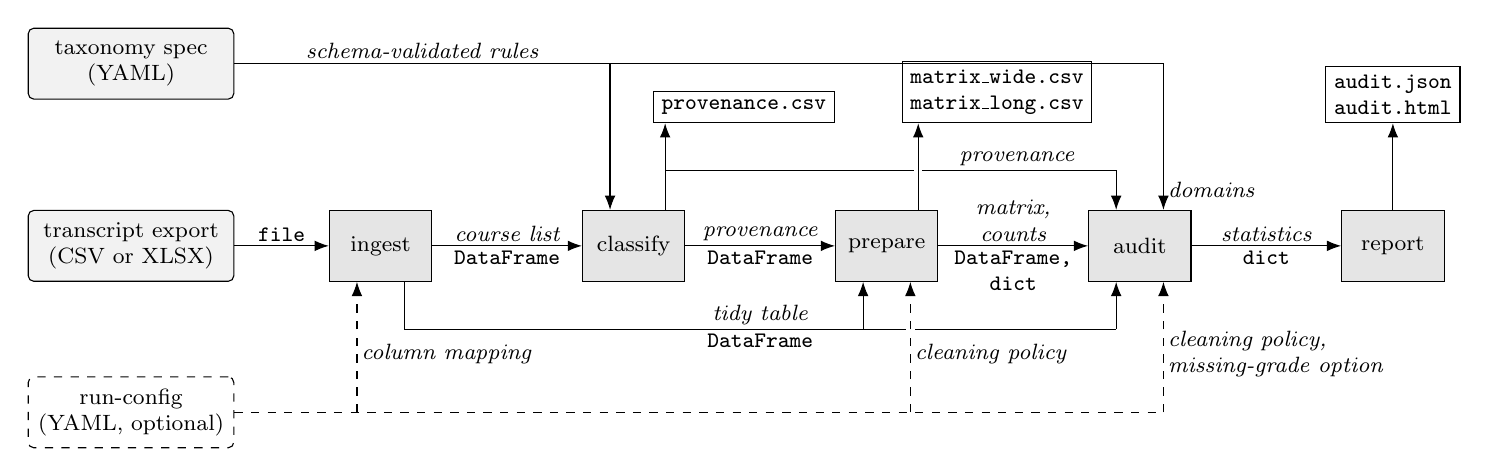
\begin{tikzpicture}[font=\footnotesize,>={Latex[length=1.8mm]},node distance=5mm and 19mm,
  inp/.style={draw,rounded corners=2pt,fill=black!5,align=center,inner sep=3pt,minimum height=9mm,text width=24mm},
  opt/.style={inp,dashed,fill=none},
  st/.style={draw,fill=black!10,align=center,minimum height=9mm,minimum width=13mm,inner sep=2pt},
  outp/.style={draw,align=center,inner sep=3pt,font=\footnotesize\ttfamily},
  lab/.style={font=\footnotesize\itshape,inner sep=1.5pt},
  fmt/.style={font=\footnotesize\ttfamily,inner sep=1.5pt},
  over/.style={preaction={draw,white,line width=3pt,-}}]
\node[inp] (tr) {transcript export\\(CSV or XLSX)};
\node[st,right=12mm of tr] (io) {ingest};
\node[st,right=of io] (cl) {classify};
\node[st,right=of cl] (pr) {prepare};
\node[st,right=of pr] (au) {audit};
\node[st,right=of au] (rp) {report};
\node[inp,above=14mm of tr] (tx) {taxonomy spec\\(YAML)};
\node[opt,below=12mm of tr] (cf) {run-config\\(YAML, optional)};
\draw[->] (tr) -- node[fmt,above] {file} (io);
\draw[->] (io) -- node[lab,above] {course list} node[fmt,below] {DataFrame} (cl);
\draw[->] (cl) -- node[lab,above] {provenance} node[fmt,below] {DataFrame} (pr);
\draw[->] (pr) -- node[lab,above,align=center] {matrix,\\counts} node[fmt,below,align=center] {DataFrame,\\dict} (au);
\draw[->] (au) -- node[lab,above] {statistics} node[fmt,below] {dict} (rp);
\draw ([xshift=3mm]io.south) |- node[lab,above,pos=0.75] {tidy table} node[fmt,below,pos=0.75] {DataFrame}
  ([xshift=-3mm,yshift=-6mm]au.south);
\draw[->] ([xshift=-3mm,yshift=-6mm]pr.south) -- ([xshift=-3mm]pr.south);
\draw[->] ([xshift=-3mm,yshift=-6mm]au.south) -- ([xshift=-3mm]au.south);
\draw[->] ([xshift=4mm]cl.north) |- node[lab,above,pos=0.89] {provenance} ([xshift=-3mm,yshift=5mm]au.north) -- ([xshift=-3mm]au.north);
\draw[->] (tx.east) -| node[lab,pos=0.25,above] {schema-validated rules} ([xshift=-3mm]cl.north);
\draw[->] (tx.east) -| node[lab,pos=0.93,right] {domains} ([xshift=3mm]au.north);
\draw[dashed] (cf.east) -- ($(cf.east -| au.south)+(3mm,0)$);
\draw[->,dashed] ($(cf.east -| io.south)+(-3mm,0)$) -- node[lab,right,pos=0.45] {column mapping} ([xshift=-3mm]io.south);
\draw[->,dashed,over] ($(cf.east -| pr.south)+(3mm,0)$) -- node[lab,right,pos=0.45] {cleaning policy} ([xshift=3mm]pr.south);
\draw[->,dashed] ($(cf.east -| au.south)+(3mm,0)$) -- node[lab,right,pos=0.45,align=left] {cleaning policy,\\missing-grade option} ([xshift=3mm]au.south);
\node[outp,anchor=south] (op) at ($(cl.north)+(14mm,11mm)$) {provenance.csv};
\node[outp,anchor=south] (om) at ($(pr.north)+(14mm,11mm)$) {matrix\_wide.csv\\matrix\_long.csv};
\node[outp,anchor=south] (oa) at ($(rp.north)+(0,11mm)$) {audit.json\\audit.html};
\draw[->] ([xshift=4mm]cl.north) -- ++(0,11mm);
\draw[->,over] ([xshift=4mm]pr.north) -- ++(0,11mm);
\draw[->] (rp.north) -- (oa.south);
\end{tikzpicture}}
\caption{Data flow. A transcript export and a taxonomy specification are required; a run-configuration file (dashed) is optional and supplies the column mapping, the cleaning policy, and the audit's missing-grade option. Arrow labels give what each arrow carries (italic) and its in-memory format (monospace). Classify reads only the course columns of the tidy table; prepare and audit read all of it, and audit re-applies the cleaning so that Cronbach's alpha uses the course grades.}
\label{fig:dataflow}
\end{figure}

\subsection{Software functionalities}

\textbf{Classification with provenance.} For every course, CurricuMap records the method (\texttt{override}, \texttt{rule}, \texttt{fuzzy}, or \texttt{unmatched}), the pattern and the text it matched, a score, and whether rules for more than one domain matched, so each matrix cell can be traced to the rules behind it, a derivation record of the kind data-provenance standards formalise \cite{provdm}. An optional fuzzy fallback (via \texttt{rapidfuzz}) assigns near-misses above a threshold. A course that matches nothing is flagged and listed in the audit rather than given a default domain, and a course code that the export uses for more than one title is reported, because its grades are pooled under the domain of its first title.

\textbf{Registrar cleaning.} The \texttt{prepare} stage drops declared sentinel grades and records without a numeric grade, resolves retaken courses under a configurable policy (keep the maximum, the mean, or the latest attempt by date), and removes students who cover fewer domains than a minimum, reporting how many records and students each step removed. It then aggregates grades to per-student, per-domain means or medians and writes the matrix in wide and long form.

\textbf{Audit.} The \texttt{audit} stage reports coverage (unmapped and ambiguous courses, courses per domain), descriptive statistics per domain, and Cronbach's alpha \cite{cronbach1951}, computed with the domain's courses as items on the cleaned grades of the students in the delivered matrix. A course a student did not take is a missing item. By default it is replaced by the course mean, which lowers alpha as the share of missing grades grows; listwise or pairwise treatment can be chosen, and the report gives each domain's share of missing grades. Alpha assumes essentially tau-equivalent items and is a lower bound to reliability rather than evidence that a domain is unidimensional \cite{cortina1993,sijtsma2009,mcneish2018}; the report states these assumptions and shows alpha without a colour grade when it rests on fewer than 30 students, where even unrelated grades can reach .70. Results are written as \texttt{audit.json} and as a self-contained \texttt{audit.html} (Figure~\ref{fig:audit}).

\textbf{Reproducibility.} Classification, cleaning, and aggregation are deterministic, and the generator is seeded. Following common practice for scientific software \cite{wilson2014}, \nTests{} tests with \covPct\% statement coverage run in continuous integration, including regression tests that run Listing~\ref{lst:run} verbatim and pin the results of Section~\ref{sec:validation}.

\subsection{Sample code snippets analysis}

The reuse contract is the taxonomy specification (Listing~\ref{lst:yaml}). It names the domains and an ordered list of rules. Each rule lists substring keywords (\texttt{any}) and/or regular expressions (\texttt{regex}), which are matched against the case-folded course title, and the first matching rule wins, so specific rules can precede general ones. Overrides assign exact titles and take precedence over rules. CurricuMap validates the file against a JSON Schema that rejects unknown keys, checks that every rule and override refers to a defined domain and that every regular expression compiles, and \texttt{curricumap validate-taxonomy} reports any error. Adopting the tool for a new curriculum means writing or adapting a specification, not code.

\begin{lstlisting}[float=!htbp,caption={Excerpt of the bundled ELT taxonomy (\texttt{elt\_yok\_2018.yaml}); lines starting with \texttt{\# ...} replace omitted lines, and inline comments are removed. Rules are evaluated in order; the pedagogy expression accepts \emph{e\u{g}itim} bare or with the endings \emph{-e}, \emph{-de}, and \emph{-in}, but not the possessive form in \emph{Beden E\u{g}itimi} (physical education). The full file has \eltRules{} rules with \eltKeywords{} keywords and \eltRegexes{} regular expressions (Table~\ref{tab:effort}).},label={lst:yaml}]
taxonomy:
  id: elt_yok_2018
  label: "ELT Teacher Education Curriculum (YÖK 2018)"
  # ... locale: Turkish (language: tr)
  domains:
    - { id: language_skills, label: "Language Skills" }
    # ... pedagogy, linguistics, literature, general_ed
  # ... match: fuzzy matching off
  rules:
    # ... rule 1: general_ed (Atatürk, Türk Dili, ...)
    - domain: literature
      any:
        - edebiyat
      regex:
        - '\bedeb(?![iı]l)'
        # ... one more
    # ... linguistics, language skills (2), pedagogy (öğretim)
    - domain: pedagogy
      any:
        - eğitimde
        # ... four more
      regex:
        - '(?<!beden )(?<!m[üu]z[iı]k )\be[gğ][iı]t[iı]m(e|de|[iı]n)?\b'
        # ... six more
    # ... a third pedagogy rule; general_ed electives
  overrides: []
  # ... defaults: unmatched courses are flagged
\end{lstlisting}

%% ============================================================
\section{Illustrative examples}
\label{sec:examples}

\subsection{A synthetic walkthrough}
\label{sec:walkthrough}

The bundled ELT taxonomy has five domains: Language Skills, Pedagogy, Linguistics, Literature, and General Education. Because real transcripts are personal data, the walkthrough uses the synthetic generator, so it reproduces exactly on any machine. After \texttt{pip install .} in a clone of the repository, two commands run the full pipeline from any directory (Listing~\ref{lst:run}): the first synthesises a transcript export for 60 students, and the second classifies, cleans, and audits it. A bundled taxonomy is named rather than given as a path.

\begin{lstlisting}[float=!htbp,caption={Running the illustrative example.},label={lst:run}]
curricumap synth --taxonomy elt_yok_2018 --out data \
    --n-students 60 --seed 7
curricumap run --input data/transcript.csv --taxonomy elt_yok_2018 \
    --out out
\end{lstlisting}

With seed 7 the generator emits \exRecords{} grade records across \exCourses{} courses. Its sentinel zeros always accompany a real grade, so the default retake policy (keep the highest grade) removes them with the retakes; declaring the sentinel value in the run-configuration file matters when a zero is a student's only grade in a course, as in the bundled sample transcript. The run produces a \mbox{60-by-5} student-by-domain matrix. All \exCourses{} courses are classified by rule, none ambiguous and none unmapped, and every decision, with its matched pattern, is recorded in \texttt{provenance.csv}. With $k=3$ courses per domain and \exMissMin--\exMissMax\% of course grades missing, Cronbach's alpha is \exAlphaLS{} for Language Skills, \exAlphaPed{} for Pedagogy, \exAlphaLing{} for Linguistics, \exAlphaLit{} for Literature, and \exAlphaGE{} for General Education (Figure~\ref{fig:audit}).

\begin{figure}[t]
\centering
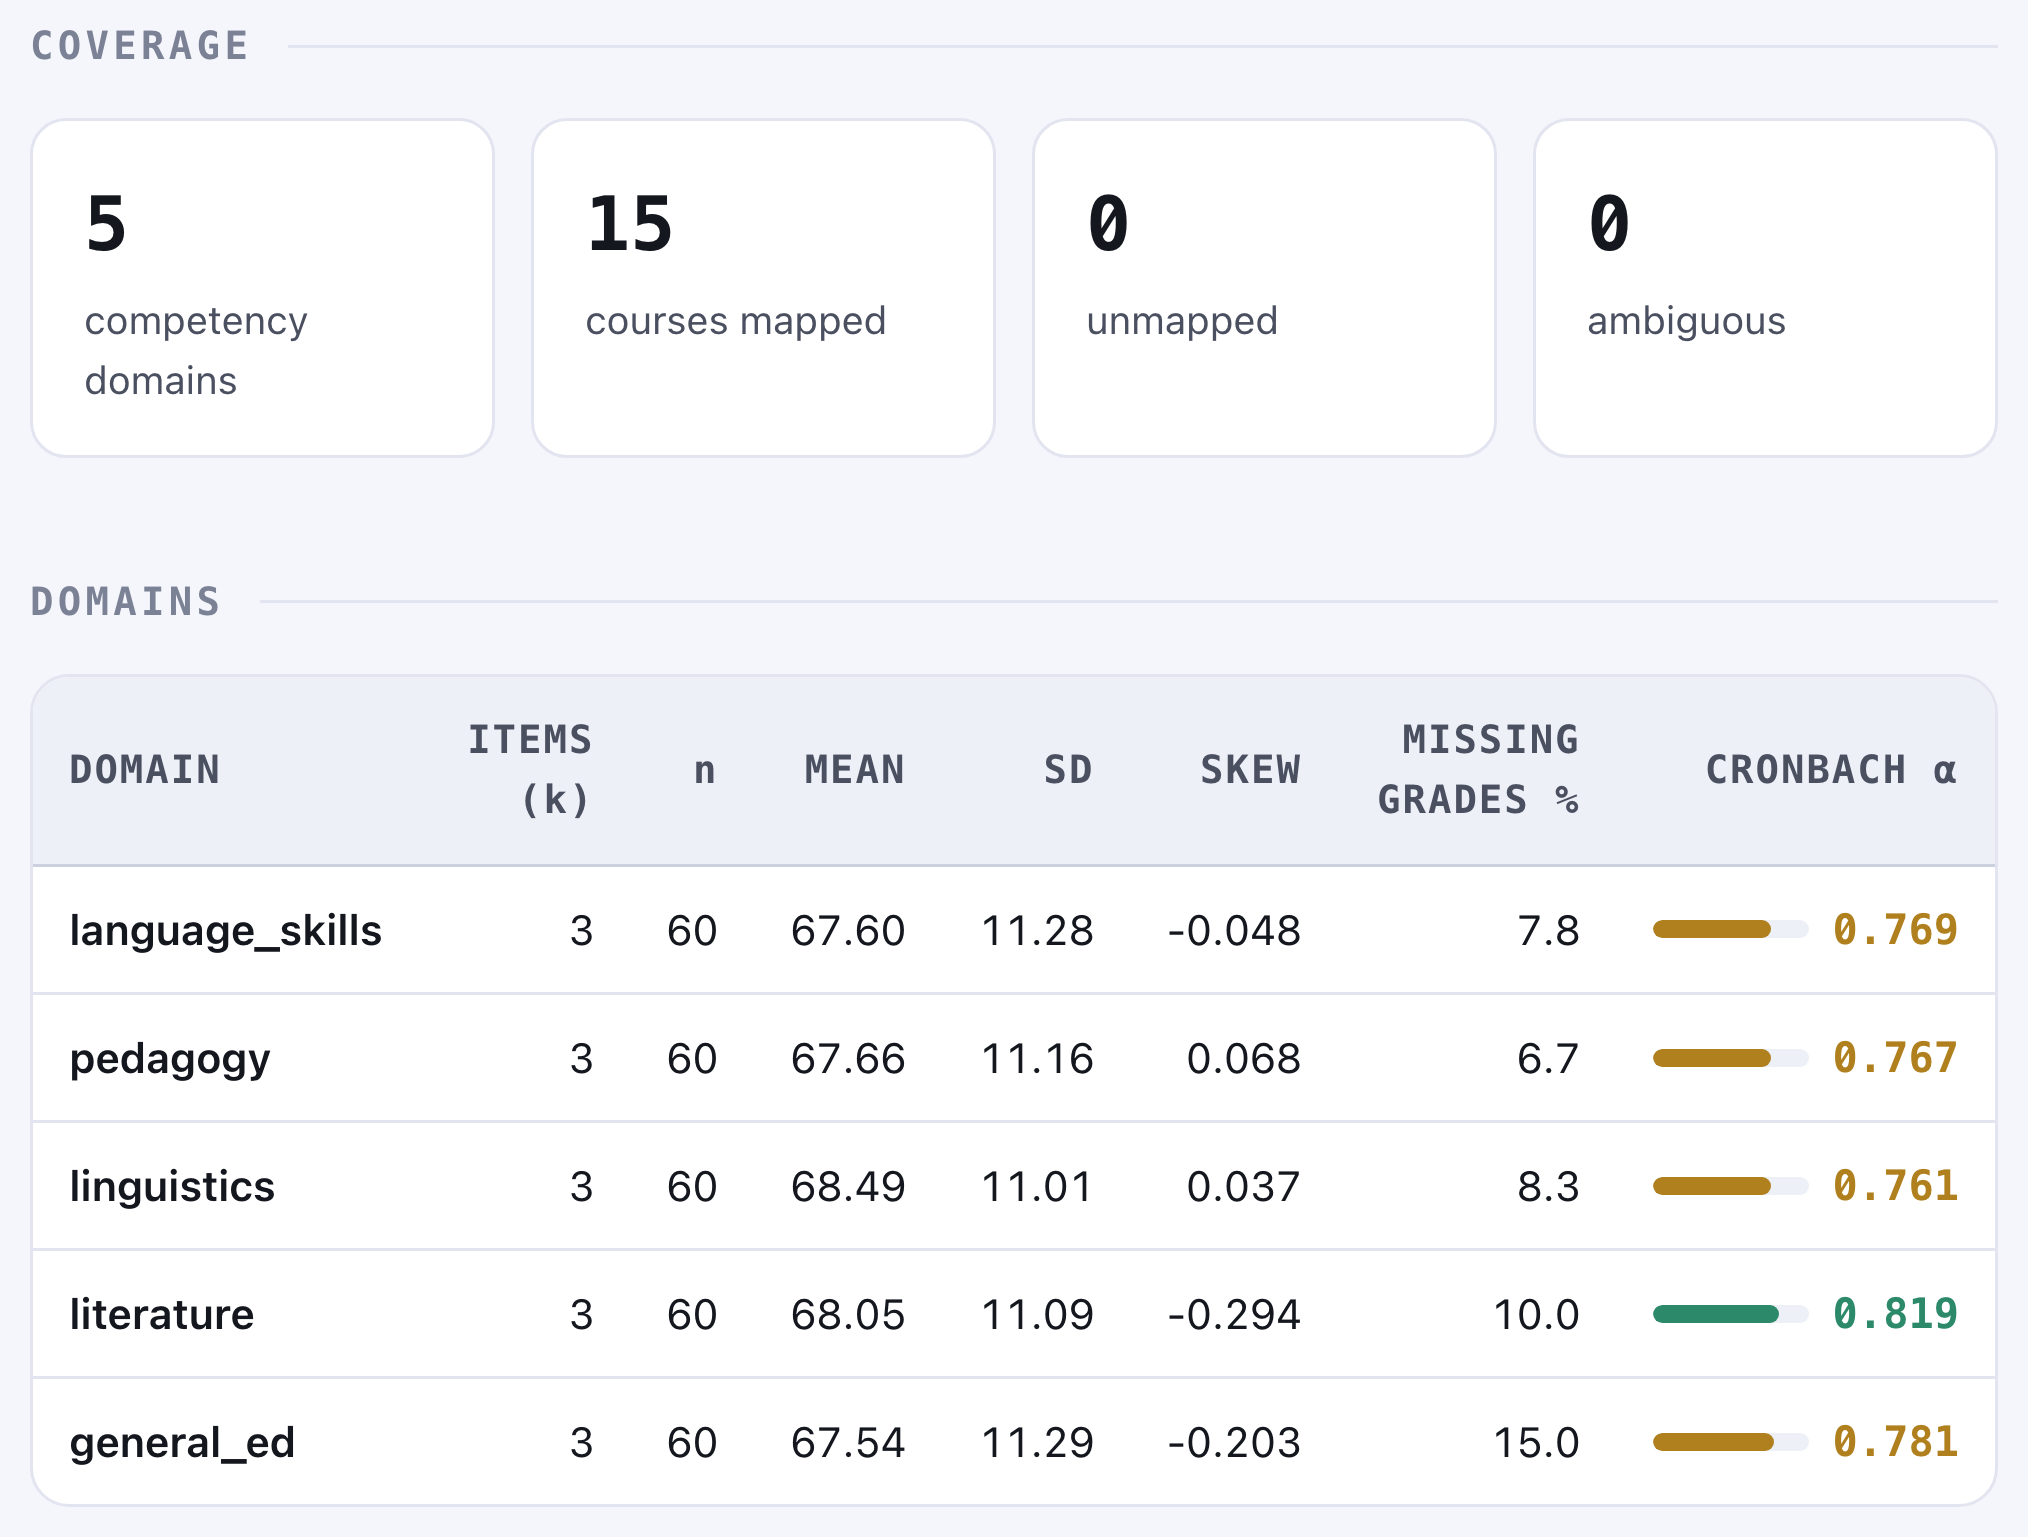
\includegraphics[width=\linewidth]{figures/fig2_audit_report.png}
\caption{Coverage tiles and domain table of the \texttt{audit.html} of the illustrative run (ELT taxonomy, seed 7, 60 synthetic students; labels enlarged for print). The bar and value of $\alpha$ are green for $\alpha \geq .80$, amber for $.70 \leq \alpha < .80$, and red for $\alpha < .70$; a negative $\alpha$ shows an empty bar with a note, and an $\alpha$ resting on fewer than 30 students is shown in grey.}
\label{fig:audit}
\end{figure}

Table~\ref{tab:bench} reports run time and peak memory of \texttt{curricumap run} on synthetic transcripts from 60 to \mbox{100{,}000} students, with catalogues of 15 or 150 courses. Below about $10^5$ grade records the time is dominated by interpreter start-up; the largest transcript, with \benchMaxRecords{} million records, is processed in \benchMaxTime~s using \benchMaxMem~MB of memory, so a programme's full history fits on a laptop.

\begin{table}[t]
\centering\footnotesize
\begin{tabular}{@{}rrrrr@{}}
\toprule
Students & Courses & Grade records & Run time (s) & Peak memory (MB) \\
\midrule
60 & 15 & 872 & 0.51 & 81 \\
1{,}000 & 15 & 14{,}716 & 0.53 & 87 \\
10{,}000 & 15 & 146{,}892 & 0.77 & 138 \\
100{,}000 & 15 & 1{,}469{,}156 & 3.19 & 412 \\
60 & 150 & 8{,}778 & 0.53 & 86 \\
1{,}000 & 150 & 145{,}912 & 0.71 & 124 \\
10{,}000 & 150 & 1{,}459{,}146 & 2.42 & 385 \\
\bottomrule
\end{tabular}

\caption{Run time (median of three runs) and peak resident memory of \texttt{curricumap run} on synthetic transcripts (generator seed 1). Each run is a fresh Python process, so the times include interpreter start-up and imports (about \benchStartup~s). Hardware: Apple M2 Max with 32~GB of memory, macOS~26, Python~3.13, pandas~3.0.}
\label{tab:bench}
\end{table}

\subsection{Validation on a real registrar catalogue}
\label{sec:validation}

We tested how a taxonomy written from curriculum documents assigns the courses of a real registrar export, what its rules add to a lookup of the labelled official titles, and how NLP and LLM classifiers given the same information compare; data, prompts, model outputs, and scripts are in the repository's \texttt{validation} directory.

\textbf{Data and reference.} The test set is the \nTitles{} distinct course titles in the 2017--2026 transcript export of the ELT programme at \.Istanbul University-Cerrahpa\c{s}a, spelled as exported, in upper case with numerals and abbreviations. After CurricuMap's normalisation, \nExact{} titles are identical to an entry of the 2018 national programme \cite{yok2018} or its 2006 predecessor \cite{yok2006}, \nVariant{} are other renderings of an entry, and \nUnseen{} are in neither programme (three local or elective courses and two versions of an official course for international students). Reference domains follow a fixed convention. Teaching-profession courses are Pedagogy, and general-culture courses are General Education; these two rules follow from the official category, which the programmes or the registrar's course codes record, and settle 79 titles. Field courses go to the domain of their subject matter, and English-language-teaching methodology courses to Pedagogy; these 62 decisions are ours. A 2006 second-foreign-language course is General Education like its 2018 successor, and a university-wide elective is General Education, a rule we added when labelling the test set. One official title, \emph{T\"urk E\u{g}itim Tarihi}, is a teaching-profession course in 2018 and a general-culture course in 2006; a title-level specification can follow only one programme, and the test set labels it by 2018. The convention, the reference labels, and the domain definitions were drafted with the help of an AI assistant (Claude, Anthropic).

\textbf{Systems.} The bundled taxonomy was drafted by an LLM coding assistant (Claude Opus~5.5 in Claude Code) from the convention and the 158 labelled entries (150 distinct titles) of the two national programmes, critiqued by three further instances (for over-fitting, false positives, and fidelity to the convention), and revised by a fifth, in 85 minutes; by design, no author edited or reviewed the rules before they were frozen. The released tool-call logs, which replay to the frozen file, show that no agent opened the catalogue, which had been moved out of the repository. Their instructions, however, were written by an assistant that had seen it: they quote one registrar variant verbatim and name two hypothetical courses resembling catalogue titles, and the reviser probed a second variant verbatim, so neither the variant nor the unseen titles are a fully blind test. The drafter, which saw none of these, had already assigned all exact and variant titles correctly, and three of the five unseen ones. Claude Code also placed a memory index and a file listing from the first author's private workspace in each agent's context; neither contains a course title, and no agent opened a listed file. The specification was frozen and applied once. The alternatives receive the labelled official titles (L), definitions of the five domains (D), or both. An exact-title lookup runs the labelled titles in CurricuMap as overrides; string similarity (\texttt{rapidfuzz}) and multilingual-E5 embeddings \cite{wang2024e5,reimers2019} assign the label of the most similar title; a character 2--5-gram logistic regression \cite{pedregosa2011} is trained on them; E5 zero-shot picks the most similar definition. Two LLMs classify every title zero-shot (D) or few-shot (L+D): Gemma~4 12B \cite{gemma4}, an open-weight model run locally in 4-bit quantisation, greedily and in five sampled runs, and Claude Opus~5.5 \cite{claudeopus55}, a proprietary model run five times through its command-line client on 1 October 2026. The definitions were also written with knowledge of the catalogue, which can only favour the systems that receive them.

\begin{table}[t]
\centering\scriptsize
\setlength{\tabcolsep}{3pt}
\begin{tabular}{@{}llrrcrrrr@{}}
\toprule
 & & & & & \multicolumn{3}{c}{Correct titles} & \\ \cmidrule(lr){6-8}
System & Input & Cov. & Acc. & 95\% CI & Exact & Variant & Unseen & $p$ \\
 & & (\%) & (\%) & (\%) & (128) & (10) & (5) & \\
\midrule
CurricuMap rules (v0.2.0) & L & 100.0 & 100.0 & 97.4--100.0 & 128 & 10 & 5 & -- \\
CurricuMap exact lookup & L & 89.5 & 89.5 & 83.4--93.5 & 128 & 0 & 0 & $<$0.001 \\
CurricuMap, v0.1.0 taxonomy & -- & 49.0 & 40.6 & 32.9--48.8 & 50 & 4 & 4 & $<$0.001 \\
String similarity & L & 100.0 & 98.6 & 95.0--99.6 & 128 & 10 & 3 & 0.500 \\
Character $n$-grams & L & 100.0 & 100.0 & 97.4--100.0 & 128 & 10 & 5 & 1.000 \\
E5, nearest title & L & 100.0 & 100.0 & 97.4--100.0 & 128 & 10 & 5 & 1.000 \\
E5, zero-shot & D & 100.0 & 68.5 & 60.5--75.6 & 92 & 3 & 3 & $<$0.001 \\
Gemma 4 12B, zero-shot & D & 100.0 & 91.6 & 85.9--95.1 & 118 & 8 & 5 & $<$0.001 \\
Gemma 4 12B, few-shot & L+D & 100.0 & 100.0 & 97.4--100.0 & 128 & 10 & 5 & 1.000 \\
Claude Opus 5.5, zero-shot & D & 100.0 & 98.6 & 95.0--99.6 & 126 & 10 & 5 & 0.500 \\
Claude Opus 5.5, few-shot & L+D & 100.0 & 100.0 & 97.4--100.0 & 128 & 10 & 5 & 1.000 \\
\bottomrule
\end{tabular}

\caption{Classification of the \nTitles{} registrar titles. Input: labelled official titles (L), domain definitions (D), both, or neither (--). Cov.: titles assigned a domain (CurricuMap flags the rest). Acc.: titles assigned the reference domain (flags count as errors), with a Wilson 95\% interval; with the \nClusters{} title stems as units (numbered courses share one), the bound for 100\% is \clusterLo\%. Correct titles per stratum ($n$): exact official titles, other registrar renderings, titles in neither programme. $p$: exact McNemar test against the first row; a difference of five titles or fewer cannot reach $p<0.05$. String similarity breaks ties by the plain ratio, a rule set after its first run's tie errors were seen. Gemma: greedy decoding; Claude: five runs with identical labels.}
\label{tab:validation}
\end{table}

\textbf{Results.} The frozen taxonomy assigned all \nTitles{} titles by rule, each to its reference domain (Table~\ref{tab:validation}). For \nAmbiguous{} compound titles, such as ``Dil ve Edebiyat \"O\u{g}retimi'' (teaching language through literature), a subject rule and a teaching rule both matched; rule order resolved each correctly, and the ambiguity flag marks them for review. The exact lookup assigned the \nExact{} exact titles and flagged the other \lookFlagged{} without error, so the rules contributed the \nVariant{} registrar variants (a lookup that also ignored punctuation, spaces, and diacritics would recover \nVariantLooseW{} of them) and the \nUnseenW{} unseen titles, which general stems (\emph{\"o\u{g}retim}, \emph{Atat\"urk}, \emph{k\"ult\"ur}) placed correctly but without a flag. The other methods given the labelled titles reached \listAccMin--\listAccMax\%, none significantly different from CurricuMap ($p \geq \listPMin$). Without them, E5 zero-shot reached \eZSAcc\% and the open-weight LLM \gmZSgAcc\% (sampled runs \gmZSAccMin--\gmZSAccMax\%, with identical labels for only \gmZSIdentical\% of the titles), both below CurricuMap (\gmZSgPt{} greedy; $p \leq \gmZSPMaxUp$ for each sampled run). The proprietary LLM reached \clZSAcc\% zero-shot (\clZSPt{} against CurricuMap), with identical labels in all \clZSRunsW{} runs; its \clZSWrongW{} errors were general-culture courses of the 2006 programme, such as ``Drama'', whose category only the programme documents settle. The taxonomy released with v0.1.0, written for synthetic data, assigned only \vOneCov\% of the titles and \vOneAcc\% correctly.

\begin{table}[t]
\centering\scriptsize
\begin{tabular}{@{}lrrrrrr@{}}
\toprule
Taxonomy & Domains & Rules & Keywords & Regexes & Overrides & YAML lines \\
\midrule
\texttt{bologna} & 3 & 3 & 14 & 0 & 0 & 19 \\
\texttt{canmeds} & 7 & 7 & 27 & 0 & 0 & 31 \\
\texttt{elt\_yok\_2018} & 5 & 9 & 53 & 63 & 0 & 159 \\
\texttt{engineering\_mudek} & 5 & 5 & 40 & 0 & 0 & 25 \\
\texttt{math\_ed\_yok} & 4 & 4 & 23 & 0 & 0 & 22 \\
\texttt{elt\_yok\_2018\_v0.1.0} & 5 & 5 & 34 & 0 & 0 & 25 \\
\bottomrule
\end{tabular}

\caption{Size of the bundled taxonomy specifications; YAML lines exclude blank and comment lines. \texttt{elt\_yok\_2018\_v0.1.0} is the ELT taxonomy released with v0.1.0.}
\label{tab:effort}
\end{table}

\textbf{Specification size.} The validated ELT taxonomy has \eltRules{} rules with \eltKeywords{} keywords, \eltRegexes{} regular expressions, and no overrides in \eltYamllines{} lines of YAML (Table~\ref{tab:effort}). Keywords alone correctly assign \eltKwOnlyCorrect{} of the \eltKwOnlyEntries{} official entries. Regular expressions assign all but one of the rest, mostly because a plain stem would also take look-alike courses (\emph{e\u{g}itim}, education, also occurs in \emph{Beden E\u{g}itimi}, physical education); the remaining entry, the 2006 \emph{T\"urk E\u{g}itim Tarihi}, needs an override. Most other regular expressions accept registrar renderings, such as ASCII spellings (\texttt{OGRETIM}) and abbreviations (\texttt{\"O\u{G}R.}).

\textbf{What the comparison shows.} Given the labelled official list, every method that generalises beyond exact titles was about equally accurate on this catalogue (\listAccMin--\listAccMax\%); only the exact lookup, which flags every title it has not seen, fell short (\lookAcc\%). Accuracy therefore does not separate CurricuMap from those methods; they differ in what they leave behind. CurricuMap executes and records whichever mapping is chosen: rules generalise to registrar renderings at a cost in readability, overrides record single decisions, and an LLM or a nearest-neighbour lookup can propose either. A hosted LLM can change or be withdrawn, identical requests can return different answers \cite{atil2025,reiss2023}, and its stated reasons are not guaranteed to be faithful or reproducible. A reviewed specification, versioned with the study, states every decision, runs identically without sending data anywhere, and is cited with the software.

\textbf{Limitations.} The test set comes from one institution that follows the national curriculum closely: \nExact{} of its \nTitles{} titles are official titles in upper case, which any method given the labelled list recognises, and only \nUnseenW{} are outside both programmes. The reference for the 62 field courses reflects our convention; no independent experts labelled the titles, so expert agreement was not measured. Rules match stems, so an off-curriculum course containing one is assigned rather than flagged: \emph{Rus Dili Dilbilgisi} (Russian grammar) would go to Language Skills through \emph{dilbilgisi}, and the provenance table, not the absence of flags, is what a reviewer must check. The rules were written by LLM agents and should be reviewed by a curriculum expert before reuse. The evaluation scores course titles, not the matrices built from them; matrix construction is tested on synthetic data.

%% ============================================================
\section{Impact}

CurricuMap removes a bottleneck in competency-level learning analytics: turning records that institutions already hold into a matrix that can be analysed and reported. For existing research questions, the main gain is that the preprocessing becomes part of the evidence: a study can cite its taxonomy file and software version, and reviewers can inspect every course assignment in the provenance table. Because a specification is a small file, a study can also rebuild its matrix under alternative course mappings and report how much its findings depend on them, in the spirit of multiverse analyses of learning-analytics pipelines \cite{tang2025}. Programmes that follow the same national curriculum can share a taxonomy and add only their local courses: the bundled taxonomy assigned all \vTwoCorrect{} course titles of one institution without any local addition (Section~\ref{sec:validation}).

Some questions may become practical, such as comparing competency profiles across institutions that share a national programme, or following the same domains across a curriculum reform. The bundled taxonomy covers both the 2006 and the 2018 Turkish ELT programmes except for the one course whose category changed between them, which needs an override for 2006 cohorts.

CurricuMap grew out of the preprocessing for two ongoing studies of English-language-teacher education by the authors, to be reported separately. Its repository was made public in July 2026, and v0.1.0 was released in August 2026. The repository, its Zenodo archive, and the open validation data allow every result here to be rerun or, for the hosted LLM, recomputed from the released outputs. We invite curriculum and learning-analytics researchers to contribute taxonomies for their own programmes.

%% ============================================================
\section{Conclusions}
\label{sec:conclusions}

CurricuMap converts a registrar transcript export and a declarative YAML taxonomy into an analysis-ready student-by-domain matrix, with per-course provenance, documented registrar cleaning, and an audit of coverage and reliability. Its contribution is not a new classifier but an explicit, versioned, and testable record of the course-to-domain mapping, executed the same way every time on local data. On a real registrar catalogue, an LLM-drafted taxonomy frozen before testing assigned all \vTwoCorrect{} course titles as its convention prescribes, as did the best alternatives given the same labelled course list, and each decision can be traced to a rule a reader can check. Future work will validate taxonomies for further programmes against independent expert labels and support LLM-assisted drafting in which an expert approves each rule.

\section*{Ethics statement}
No ethics approval was required: the study uses only the course titles of the programme's 2017--2026 transcript export, extracted locally, and releases only course-level information. No student data were shared, including with the hosted language model.

\section*{Data availability}
The source code, the five taxonomies, and the validation data (course titles, registrar course codes, official categories, reference labels, prompts, raw model outputs, and all predictions) are openly available under the MIT licence (Table~\ref{tab:codemeta}). Student-level transcript records are confidential and are not shared; the synthetic generator reproduces every example without them.

\section*{Declaration of competing interest}
The authors declare that they have no known competing financial interests or personal relationships that could have appeared to influence the work reported in this paper.

\section*{Funding}
This research did not receive any specific grant from funding agencies in the public, commercial, or not-for-profit sectors.

\bibliographystyle{elsarticle-num}
\bibliography{references}

\end{document}
